\section{Histogram: Seeing the Shape of Your Numbers}

Imagine you’re organizing a large set of test scores from a group of students. You want to see how the scores are distributed: Are most students scoring in the 80s, or is there a wider spread?

A histogram is like a map of all the test scores, showing you where the majority of students are scoring and how the scores spread out across different ranges.

\subsection*{Key Concepts: Let’s Explore!}

\textbf{Numerical Data: Numbers are Key!}

Numerical data can represent things like: 
\begin{itemize}
    \item Test scores
    \item The amount of time spent studying
    \item The number of goals scored in a match
\end{itemize}

\textit{Activity: Can you think of three other examples of numerical data you use regularly?}

Histograms are specifically for numerical data. Why do you think histograms are used for numbers and not for things like colors or types of fruit? (Hint: Numbers have an inherent order, and you can compare them to each other more easily.) \newline

\noindent\textbf{Bins (Intervals): Grouping for Clarity}

Imagine breaking the range of test scores [0,100] into bins, or groups. For example, one bin might represent scores from 0 to 10, another from 11 to 20, and so on. These bins help us organize the data into manageable chunks. \newline

\textit{Activity: Why do you think we group the data into bins? What would happen if we had a “bin” for every single score, especially with a large number of students?} (Hint: If you have too many bins, it can be hard to see the patterns clearly.) \newline

Why do you think it’s better to keep the width of each bin the same? (Hint: Consistent bin widths make the histogram easier to read and compare.) \newline

\noindent\textbf{Frequency: Counting What Falls Where}

Once we’ve grouped the scores into bins, we count how many students fall into each range. This is called frequency. For example:
\begin{itemize}
    \item 5 students scored between 0–10,
    \item 12 students scored between 11–20,
    \item 10 students scored between 21–30.
\end{itemize}

\textit{Activity: If you have more students in one bin than another, what does this tell you about the scores in that range?} \newline

\noindent\textbf{Bars: Visualizing the Counts}

We then draw a bar for each bin, where the height of the bar represents the frequency (how many students scored in that range). \newline

\textit{Activity: If one bar is much taller than another, what does this mean?} (Hint: A taller bar shows a higher frequency, meaning more students scored in that range.)\newline

\noindent\textbf{Shape of Distribution: Unveiling Patterns}

The overall shape of the histogram reveals key insights about the distribution of the data. Let’s look at some common shapes:

\begin{itemize}
    \item \textbf{Symmetry or Skewness:}
    \begin{itemize}
        \item \textit{Symmetric:} Imagine the histogram looks like a bell curve (a normal distribution). This suggests the data is evenly distributed, with most students scoring around the middle.
        \item \textit{Skewed:} What if the histogram is lopsided, with a long tail on one side? Skewed data often has outliers that pull the data to one side, such as a few students with very high or very low scores.
    \end{itemize}
    \item \textbf{Central Tendency:} The center of the histogram (where the highest bars are) gives us a sense of where most of the data lies. The center is often close to the average, or mean, of the data.
    \item \textbf{Spread or Variability:} A wide histogram with bars spread across many bins suggests that the data has a wide range of values. A narrow histogram shows the data is concentrated around one main value.
    \item \textbf{Modality:}
    \begin{itemize}
        \item \textit{Unimodal:} A histogram with one peak suggests that most data points group around one central value.
        \item \textit{Bimodal:} A histogram with two peaks suggests two distinct groups in the data.
    \end{itemize}
\end{itemize}

\textit{Activity: Can you think of a situation where a bimodal distribution might occur?} (Hint: If you have data from two groups, like the test scores of two different classes with very different performance levels, you might see two peaks.)

Now let’s explore the climate dataset and visualize histogram using R.

\subsection*{Pressure Distribution using Histogram}

\begin{verbatim}
histogram(~ Pressure, df_climate,
          main = "Distribution of Atmospheric Pressure",
          xlab = "Pressure (hPa)",
          ylab = "Frequency",
          breaks = 30)
\end{verbatim}

% Figure here -------------------------
\begin{figure}[h!]
    \centering
     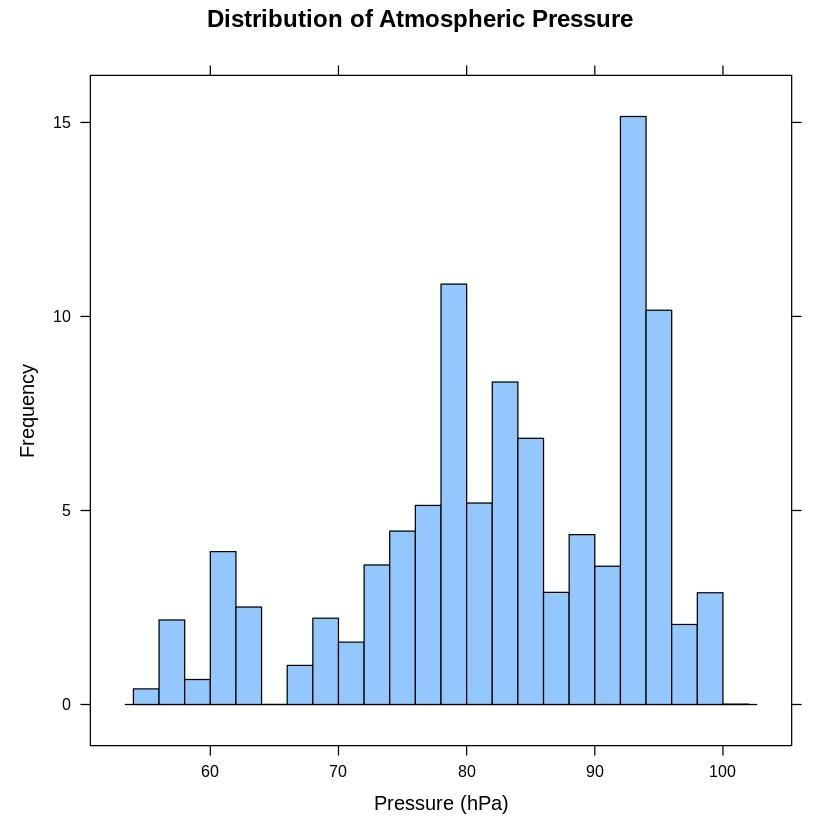
\includegraphics[width=0.6\textwidth]{figures/hist1.jpg}
    \caption{Pressure Distribution using histogram}
\end{figure}


\subsection*{Wind Speed Distribution Analysis with Density Curve}

\begin{verbatim}
# Create histogram with density curve
ggplot(df_climate, aes(x = WindSpeed_10m)) +
  geom_histogram(aes(y = after_stat(density)), bins = 30, 
  fill = "skyblue", color = "black", alpha = 0.7) + 
  geom_density(color = "blue", linewidth = 1) + 
  labs(title = "Histogram of Windspeed with Density Trendline ",
       x = "Temperature (°C)",
       y = "Density") +
  theme_minimal()
\end{verbatim}

% Figure here --------------------------
\begin{figure}[h!]
    \centering
     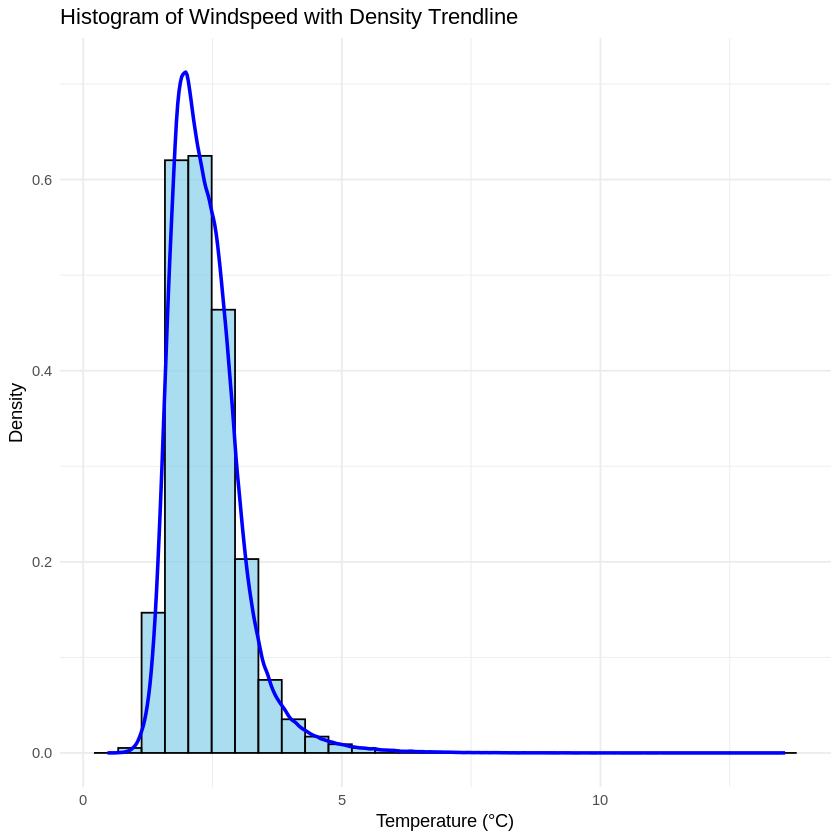
\includegraphics[width=0.5\textwidth]{figures/hist2.png}
    \caption{ Windspeed with Density Trend}
\end{figure}
